%%% Template originaly created by Karol Kozioł (mail@karol-koziol.net) and modified for ShareLaTeX use

\documentclass[a4paper,11pt]{article}
\usepackage[T1]{fontenc} %thanks's daleif
\usepackage[utf8]{inputenc}
\usepackage[english, danish]{babel}
\usepackage[T1]{fontenc}
\usepackage[utf8]{inputenc}
\usepackage{graphicx}
\usepackage{xcolor}
\graphicspath{ {image/} }
\usepackage{tgtermes}

\usepackage[
pdftitle={Opgave 5}, 
pdfauthor={Ole Schultz, DTU Diplom Informatik},
colorlinks=true,linkcolor=blue,urlcolor=blue,citecolor=blue,bookmarks=true,
bookmarksopenlevel=2]{hyperref}
\usepackage{amsmath,amssymb,amsthm,textcomp}
\usepackage{enumerate}
\usepackage{multicol}
\usepackage{tikz}

\usepackage{geometry}
\geometry{total={210mm,297mm},
left=25mm,right=25mm,%
bindingoffset=0mm, top=20mm,bottom=20mm}


\linespread{1.3}

\newcommand{\linia}{\rule{\linewidth}{0.5pt}}

% custom theorems if needed
\newtheoremstyle{mytheor}
    {1ex}{1ex}{\normalfont}{0pt}{\scshape}{.}{1ex}
    {{\thmname{#1 }}{\thmnumber{#2}}{\thmnote{ (#3)}}}

\theoremstyle{mytheor}
\newtheorem{defi}{Definition}

% my own titles
\makeatletter
\renewcommand{\maketitle}{
\begin{center}
\vspace{1ex}
{\huge \textsc{\@title}}
\vspace{1ex}
\\
\linia\\
\@author \hfill \@date
\vspace{3ex}
\end{center}
}
\makeatother
%%%

% custom footers and headers
\usepackage{fancyhdr,lastpage}
\pagestyle{fancy}
\lhead{}
\chead{}
\rhead{}
\lfoot{Opgave \textnumero{} 5}
\cfoot{}
\rfoot{Page \thepage\ /\ \pageref*{LastPage}}
\renewcommand{\headrulewidth}{0pt}
\renewcommand{\footrulewidth}{0pt}
%

%%%----------%%%----------%%%----------%%%----------%%%

\begin{document}

\title{Opgave 5 adc-pwm lysstyring}

\author{Ole Schultz Dtu Diplom Informatik}

\date{14/11/2017}

\maketitle

\section{Formål}
Formålet med opgaven er at:
\begin{itemize}
 \item Skrive et struktureret program i C med passende antal c-moduler der kan styre lysstyrke eller motors hastighed - alternativt servorer på MeArm
\end{itemize}

\subsection{Læringsmål}
\begin{itemize}
\item At lære at programmere ADC-konverter i Atmega2560 op og at anvende ADC konverteren, med Free Running/single sample og i auto trigger-mode hvor adc-samplings hastigheden styres af et timer interrupt.
\item  At kunne sende adc samples, der konverteres til en spænding og repræsenteres i ascii, op på en PC-terminal vha. en UART.
\item Fra PC-terminalen at kunne modtage en streng med information om minimum - og maksimum for pulsebredde og kunne oversætte dem fra ascii til binær/decimal, så de kan bruges i programmet til til at styre grænsen for pulsbredden på PWM-signalet
\item At kunne anvende en switch case eller anden implementation af en tilstandsmaskine for at styre den ADC kontrollerede PWM styring af LED lys eller servo-motor.
\item At kunne skrive et strukturelt c-program med passende moduler – min. et modul for hver hardware-enhed i Atmegaen, der benyttes i programmet.
\item At kunne dokumentere det samlede program i en rapport
\end{itemize}
\subsection{Specifikation:}
\begin{itemize}
\item Et analogt signal gennem ADC-input styrer pulsebredden (PWM signal)
\item PWM signalet skal aktiveres på passende udgang i Mega’en
\item PWM signalet forbindes til en LED’s – så lysstyrken kan varieres vha. et potentiometer sat til adc-indgangen eller en/flere servo motorers hastigheder – MeArm robot arm.
\item Der skal via UART og PC-terminal kunne sættes min. og maks. grænser for lys styrken
\item Hvis du arbejder med styring af servo motorer så skal der via uarten gives kommandoer til servoerne – dvs. styrer armens bevægelse.
\end{itemize}

%\begin{defi}
%The \textbf{complex number} $z$ is a number that can be expressed in the form
%\begin{equation}
%z = a + bi\ ,
%\label{r1}
%\end{equation}
%where $a, b \in \mathbb{R}$ and $i$ is an \textbf{imaginary unit}, defined as:
%$$i=\sqrt{-1} \qquad \text{or} \qquad i^2= -1\ .$$ 
%\end{defi}

\subsection{Dokumentation}

Skriv en rapport der tager udgangspunkt i rapport templaten– det er på Campusnet under dokumentation. Der skal være:
\begin{itemize}
\item et c-modul diagram med forklaring,
\item interrupt diagram med forklaring,
\item flow chart for int main() eller tilstands diagram med forklaring –
for hvert modul en tabel med funktioner og beskrivelse af hvad de gør
\item del-test resultater – og slut test resultater
\item en konklusion!
\end{itemize}
Se dokumenterne: documentation\_equirements\_for\_embedded\_C.pdf og eksempel
– Koden evalueres og rapporten rettes og disse indgår i den endelige bedømmelse ved den mundtlige eksamen

\subsection {Aflevering}
\begin{itemize}
\item Et zippet AtmelStudio projekt og en rapport i PDF format d. 9.Dec ellers ingen adgang til eksamen
\item Forudsat læst afsnit i bogen s. 621 -626 16 – 16.2.4, s. 628 -639 16.2.7 – 16.3, slideserier med tilhørende video for lektion 10 og 11 og mens du skriver koden læs manual s. 275 - 283, og 288-295,
\end{itemize}


\clearpage

\section{Lysstyring}
Blok diagram vover  niveau systemet på koncept
\paragraph{}
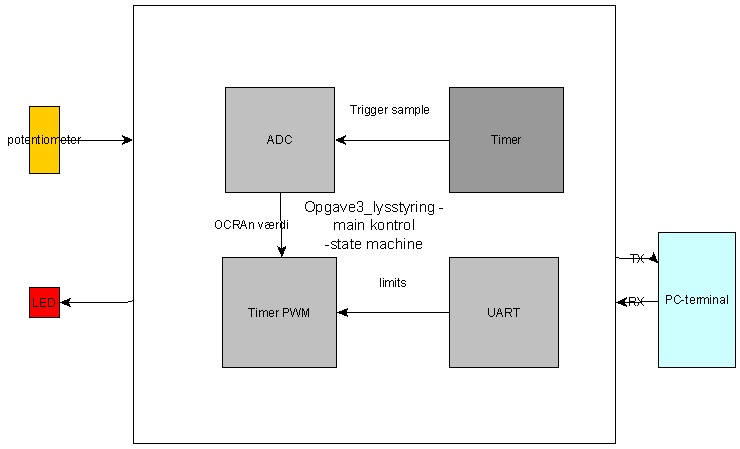
\includegraphics[scale=0.8]{koncept}

\paragraph{Detail Specifikation:}
\begin{enumerate}[(a)]
\item  Terminal skal bruges som input med grænser for PWM til styringen. Så at der kan sættes en grænse værdi for mindste - og maks. lysstyrke, der kan skrues op/ned vha. en variabel ekstern spænding (0-3.3V) på adc-input. 

\item  DC skal læse på en adc-input kanal og selve adc’ens clock frekvens skal sættes med Fcpu skalleret ned til 125kHz for 10bit opløsning eller til 1 MHz- hvis der kun benyttes 8 bit samples. Se s. 271 i datablad. 
\item  Styr adc’en med interrupt on sample ready, når sample er klar i ADCL og ADCH skal adc’en give interrupt 

\item  Timer1 overflow interrupt skal styre sample raten. Sampleraten sættes til en frekvens på f.eks. 9500 Hz eller adc skal sættes op til at køre i auto-trigger mode – se datablad for mega’en

\item  Samples fra ADC’en skal testes for at være indenfor indtastede min. og maks. Når det virker så skal 

\item  adc- værdien bruges til at styre pulsbredden for en eller flere PWM’en. 

\item   PWM timer skal sættes op til at køre fasekorrekt mode eller fase og frekvens korrekt mode. 

\item  UART: Baud rate 19200, 8 data bit, 1 stop bit og ingen paritet 
\end{enumerate}

\section{bilag}
Nedenstående vejledning er ment som en hjælp, men du behøver ikke at følge den, blot at delmålene opfyldes!
\begin{enumerate}
\subsection{lektion 10}
\item  {Lav et nyt projekt ADC i Atmel Studio for adc-konvertering.}
\item {Skriv nu et program der kan initialisere ADC’en til at arbejde med single ended mode input, single running mode (ADATE bit=0 i ADCSRA register) – clock frekvens 16MHz skalleret med faktor 128, adc-kanal 0 og 5V reference ved at vælge AVCC som reference.}
\begin{enumerate}
\item [a.] Skriv en initialiserings-funktion – der sætter relevante bit i ADMUX, ADCSRA, ADCSCRB, DIDR0.
\item [b.] Kald adc initialiserings-funktionen fra int main() og brug simulatoren til check af, at de rigtige bit er blevet sat i registrene.
\end{enumerate}
\item Skriv en funktion unsigned int getSample(unsigned char channel) i adc-modulet, der kan returnere en sample for en channel, når ADIF bit går højt i ADCSRA registeret – se flow chart 


\begin{center}

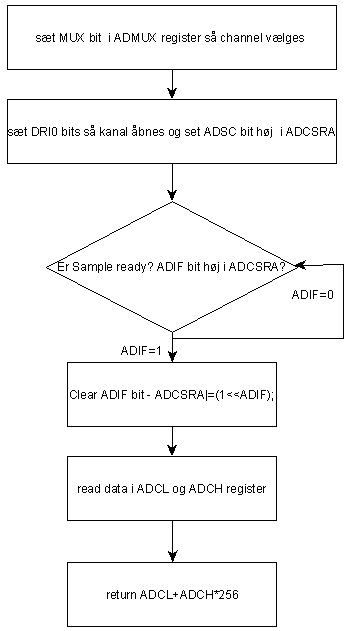
\includegraphics[scale=0.7]{adc_getSample}

\end{center}
\par –Husk i single mode, så skal programmet sætte ADSC=1 i ADCSRA registeret! for hver gang man ønsker en ny sampling.
\item Forbind et potentiometer mellem gnd og 3.3 V og forbind midter-benet til den adc kanal du har valgt.
\item Når dette kode kompilerer, så kald funktionen getSample(0),(0 når A0 pind benyttes) indefra while(1) løkken i main() med et interval på 100 ms. Det medfører at sample frekvens er ca. på 10Hz. - husk variablen til at modtage retur-værdien eks. \color{blue}{ unsigned int sample= getSample(0);}\color{black} //kanal 0 
\item Test:  hvis sample værdi er >=200 så tænd LED på PB7 ellers slukket. 
Skru op og ned og så skulle du gerne se, at der kommer samples ind –LED’en vil tænde og slukke.
\item	Når overnævnte virker så flyt koden under pkt. 2 for addc’en over i et c-module (adc.c og header-file adc.h). Så det indgår i strukturen.
\item  For at modtage en en sample benyttes polling princippet vha. funktionen unsigned int getSample(unsigned char channel). Men for at udnytte hardwaren bedst skal adc complete sample interrupt benyttes
 \begin{enumerate}
\item[i.]Interrupt enables ved at sætte bit ADIE bit højt i ADCSRA registeret. 

\item[ii.]	Skriv interrupt service routinen (vektor navn (ADC\_VECT)). 

\item[iii.] Enable globalt interrupt sei(); 

 \end{enumerate}
 Inde i service rutinen skal ADCL og ADCH læses ind i en global variable eks. sample og der sættes en globalt kontrol variable eks. adc\_flag=1, Flaget bruges i int main() til at teste på og når adc<\_flag=1, så kan sample f.eks.  benyttes i int main() til at tænde slukke LED på PB7.
 
 \paragraph{}Hvilken spænding repræsenterer samplen?

\item Som en option: Skriv nu i int main() eller i en selvstændig funktion den nødvendige kode, så den samplede værdi fra indgangen repræsenteres som spænding med enheden volt. Test at uart’en kan skrive spændinger ud på terminalen. Dette spørgsmål er en option – du lærer mere og risikerer at få en højere karakter! 

\item Da compileren ikke understøtter floating point direkte uden integration af ekstra compiler optioner skal du her lære at bruge en algoritme – Se bogen s. 638 -639 – der er et eksempel – gennemgås i lektion 10. 
\subsection{lektion 11-12: PWM og interrupt styring af samplerate}
Næste opgave er nu at skrive et modul for en timer, der kan genere PWM – phase korrekt måde - jfr. Manual p. s 126 i data blad og i Huang bog læs side s. 391- 393 og eksempel s. 394-395 – gennemgås i lektion 11. Du må gerne her selv vælge timer og pwm mode som du har lyst og så kan nedenstående punkter 11 – 14 ikke benyttes direkte. 
\item	I dit Atmel studio projekt inkluderer du nu en c-file og header file for et timer c-module– der skal indeholde koden til timer PWM delen. Vælg timer0 hvis du bruger eksemplet i Huang-bogen . Skriv en funktion til initialisering af PWM fase korrekt mode. 
\begin{enumerate}
\item[a.] 	For fase korrekt mode sættes timeren for mode 1, jfr. Datablad s. 131- ved sætte WGM0 bit højt i TCCR0A registeret og hvor opdatering af sammenligningsregisteret skal gøres, når tæller når TOP (0xFF). 
\item[b.] PWM Frekvensen \[ F_{CO}=  \frac{F_{clk}}{N\*500} \] vælger du selv med en passende prescaling N   jfr. Datablad s. 127  excel file calculators for timers i PWM uploaded på campusnet under slides for lektion 11

\item[c.] 	OCRA0 værdien kan sættes til f.eks. 100 som startværdi.
\item[d.] 	Enable PWM udgang (OC0A output - PB7 – led på pind13) initialiseres i timeren ved at sætte COM0A1 høj i TCCSR0A registeret og retningen til udgang! 
\item[e.] 	Vælger du en anden timer(ere), så find hvilken pind timeren bruger som udgang og forbind en diode med for-modstand til det ben eller din servo motor(er) 
\end{enumerate}
\item  Hvis timer0's PWM virker så vil dioden lyse tilsluttet PB7. Kompiler koden med forskellige værdier skrevet til OCR0A f.eks. 2 og se lyset er svagere. Er der problemer, så brug uarten som test – udlæs passende værdier ud på PC-terminalen 

\item	Nu skal adc-konverterens samplede værdi bruges til at opdatere OCRA0 registeret, derved fås en variable PWM –Bemærk jfr. Huang-bog og datablad så kan OCRA0registeret kun opdateres, når tælleren når top-værdien. 
\item 	Når det kompilerer, så skal du uploade det i boardet og prøv at dreje på potentiometeret, så skulle lyset gerne gå op og ned i styrke – gå ned i lab eller lån et pico scope og se signalet på pind 13 på boarded. Hvorfor går lysstyrken det op og ned flere gange når du skruer potentiometeret fra den ene ende til den anden? Tag et billede eller flere, som dokumentation for at det virker

\item Nu er det tid til at definere jeres projekt og få en god struktur på main()
Hvis du ikke allerede har gjort det, så skal du designe og implementere en tilstandsmaskine for kontrol af systemet. \par Hvilke tilstande skal der til for – sekvensen fra indlæsning af grænser for PWM timer0’s 
OCR0A sammenligningsværdier, sampling, brug af samples til opdatering af OCR0A værdi med indlæsning af nye grænser – hvilke kontrol variable er nødvendige og skal erklæres i programmet? Start med at tegne tilstandsdiagram og opskriv en State transition tabel action/funktionskald tabel. 
\item 	Skriv en switch case eller en anden form for kontrol struktur, der kan implementere tilstandsmaskinen. 

\item 	Forudsat at adc’en kører med en sample complete interrupt, så lad nu adc’en køre i auto trigger mode dvs. ADAE bit skal sættes til 1 i ADCSRA registeret og aktiver timer1 on timer overflow for auto-trigger mode. 

\item 	Og lad nu timer1 styre intervallet for, hvornår der skal samples – skriv en funktion til initialiserer timeren. Den skal kører i normal mode og aktivere interrupt på timer overflow – skriv tilhørende service rutine. Der skal ikke foretages noget i service rutinen! Eksperimenter med hvor hurtigt interrupt kan køre for at PWM’en kan nå at blive opdateret -et godt gæt er på 104 usec. For 10 bit – hvorfor det? NB! 10 bit’s opløsning og med prescaller 128 

\item 	Opdater tilstandsmaskinen og test at det virker. 

\item 	Sidste punkt er at få indlæst grænserne for sammenligningsværdier fra terminalen til PWM timeren og få brugt disse i tilstanden hvor PWM timeren får opdateret sit OCR0A register. Her kan du bruge, det du lærte i opgave 3 omkring initialisering af uret. 

\item Test at systemet virker – lav en lille video i MP4 format og tag passende billeder til dokumentation i rapporten af at det virker. 
\end{enumerate}\\

Bemærk: Pkt. 15 til 21 kan være springes over, hvis du ikke har tid, men karakteren kan afhænge af det.\\




God arbejdslyst \\

2017-11-14 Ole Schultz



\end{document}
